In this section, we measure the bandwidth overheads of {\sys} for two different applications using our traffic shaping simulator (see \Cref{sec:eval-simulator}).
We present two case studies. 
First, we examine a video streaming service, which serves as a representative example of applications characterized by high sensitivity values due to the substantial fluctuations in traffic rates typically observed in video applications.
Second, a typical web service, representing applications with smaller value for sensitivity.
In both applications, a client initiates a bidirectional communication with the server to retrieve content.
We apply traffic shaping in both directions, customizing the parameters to match the traffic characteristics specific to each direction of communication.


\subsection{Case Study: Video Streaming}\label{subsec:eval-bw-video}
In this section, we examine the effect of different privacy settings on bandwidth overhead for video streaming clients.

We run experiments with three values of the DP measurement interval $\dpintvl$ for the server:
100ms, 500ms, and 1s, and we use $\ssens = 1 MB$ and $\varepsilon_{\winlen} = 1$.
For all experiments, we set the DP parameters for client request traffic as follows: $\ssens = 200$~bytes, $\winlen = 1s$, $\dpintvl = 100ms$, and $\varepsilon_{\winlen} = 1$.
For the server responses, we configure DP parameters as follows: $\ssens = 1 MB$~bytes, $\winlen = 5s$, $\dpintvl = 1 s$, and $\varepsilon_{\winlen} = 1$.
We use different set of parameters for communication from server to client and vice versa due to the different characteristics of traffic in each direction.
Periodically, at intervals of 5 seconds, client sends a small web request  to the server to download next segment of the video. 
In the reverse direction, server transmits segments to the client one by one.
Compared to the small client's request, segments are larger and have bursty traffic pattern.
As the client requests each segment preemptively, as long as the server delivers next segment within the 5 seconds, the client can play video seamlessly. 
We run experiments with 1, 16, and 128 video clients; each client requests one video randomly selected from the dataset.
For each set of configurations, we measure the per-flow relative bandwidth overhead for the video streams in the simulator.


\begin{figure}[t]
  \centering
  \begin{subfigure}{0.49\columnwidth}
      \centering
      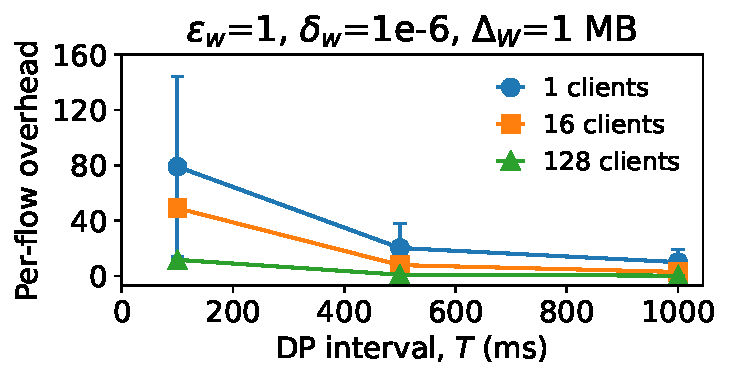
\includegraphics[width=\textwidth]{plots/overhead_vs_dp_interval_video.pdf}
      \caption{BW overhead vs DP interval (video)}
      \label{fig:video-overhead-vs-dpInt}
  \end{subfigure}
  \hfill
  \begin{subfigure}{0.49\columnwidth}
      \centering
      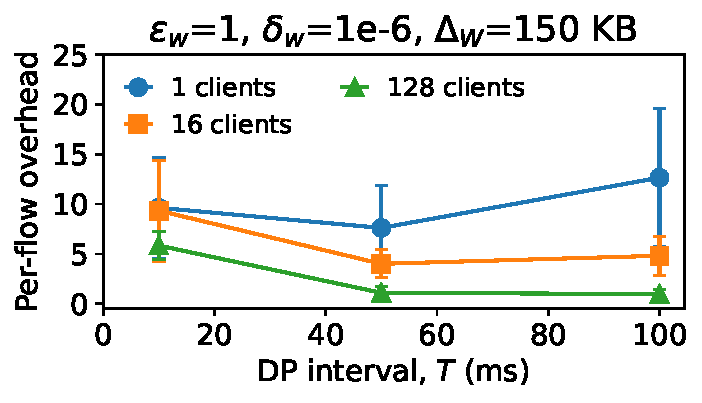
\includegraphics[width=\textwidth]{plots/overhead_vs_dp_interval_web.pdf}
      \caption{BW overhead vs DP interval (Web)}
      \label{fig:web-overhead-vs-dpInt}
  \end{subfigure}
  \caption{Video Streaming and Web Service; Bandwidth overhead for different values of DP interval.
  }
\end{figure}


\begin{figure}[t]
  \centering
  \begin{subfigure}{0.49\columnwidth}
      \centering
      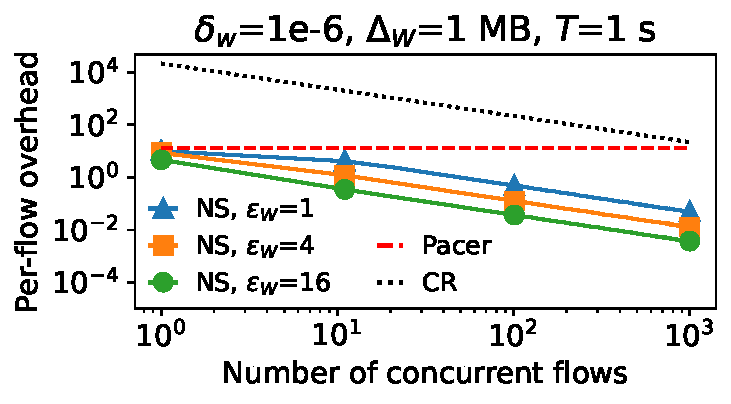
\includegraphics[width=\textwidth]{plots/overhead_vs_number_of_traces_video_loglog.pdf}
      \caption{Video streaming.}
      \label{fig:video-overheads-compare}
  \end{subfigure}
  \hfill
  \begin{subfigure}{0.49\columnwidth}
      \centering
      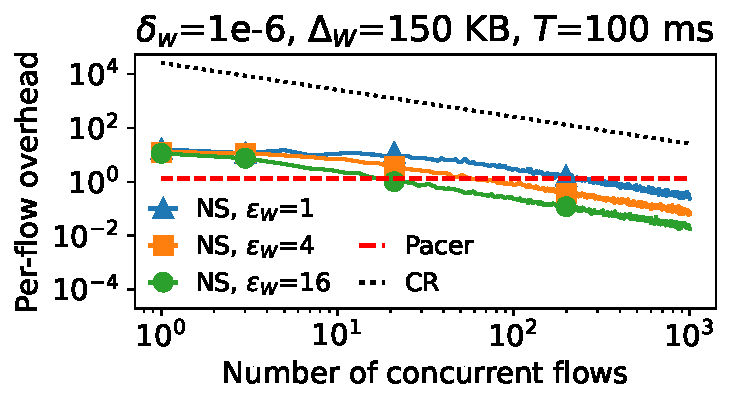
\includegraphics[width=\textwidth]{plots/overhead_vs_number_of_traces_web_loglog.pdf}
      \caption{Web service.}
      \label{fig:web-overheads-compare}
  \end{subfigure}
  \caption{Relative bandwidth overheads of {\sys} ({\ns}), constant
      shaping ({\constshape}), and Pacer.
  }
\end{figure}


\paragraph{Bandwidth overhead.}
\Cref{fig:video-overhead-vs-dpInt} shows the average per-flow relative bandwidth overhead as a function of different intervals and for varying number of clients.
The relative bandwidth overhead of a video is the number of dummy bytes transmitted normalized to the size of the unshaped video stream.
The error bars show the standard deviation in latency and bandwidth overhead.
We observe that the relative overhead decreases with larger values of $\dpintvl$.
While our simulation does not allow for the direct measurement of end-to-end latency, it's important to note that larger values for $\dpintvl$ result in data transmission occurring at more extended intervals, which can contribute to increased latency.
Therefore, the results show the trade-off between latency and bandwidth. 
A larger DP measurement interval implies higher download latency but fewer measurements and lower noise added to the payload, thus yielding a lower bandwidth overhead.
Thirdly, with multiple concurrent streaming clients, the bandwidth overhead is amortized.
Overall, {\sys}'s shaping can secure video streams with low bandwidth overheads.


\paragraph{Comparison with other techniques.}
\Cref{fig:video-overheads-compare} shows the per-flow relative bandwidth overhead of {\sys} ({\ns}) for video streaming application for varying with number of concurrent flows and for different values of $\varepsilon_{\winlen}$.
Except $\varepsilon_{\winlen}$, we use the same of parameters that we proposed in the beginning of this section.
We also compare with the overheads~that would be incurred due to constant rate
shaping ({\constshape}) and~Pacer \cite{mehta2022pacer} (see \Cref{subsubsec:background-defenses-pacer}), a SOTA system
that traffic shaping on a per-client request basis.

For {\constshape}, we configure the peak load for video service corresponding to
transmitting 1.7MB in every 5s, which is corresponding to transmitting the largest segment size in our video dataset. In other words, the {\constshape} mechanism always sends data at the maximum rate required to send a segment in our dataset.
In Pacer, for video service, we pad a segment at $i$\textsuperscript{th} index
in a video stream to the largest segment size at that index across all videos in the dataset. 
Even with the lowest privacy loss, $\varepsilon_{winlen}=1$, {\ns} add the same level of overhead as Pacer and 3 orders of magnitude less overhead than {\constshape}.  
Besides that, {\ns} can further amortize its overheads
among multiple concurrent streams within the tunnel without compromising privacy.





\subsection{Case Study: Web Service}\label{subsec:eval-bw-web}
In this section, we examine the effect of different privacy settings on bandwidth overhead for a web service.
We   
As we mentioned, we expect the values of DP measurement interval affects the communication end-to-end latency.
We choose smaller values for $\dpintvl$ for web service as compared to video streaming applications as web applications are delay-sensitive.
For the server responses, we use three values for DP measurement intervals, $\dpintvl$: 10 ms, 50 ms, 100 ms, and configure other parameters as follows: $\ssens = 150 KB$, $\winlen = 1s$, and
$\varepsilon_{\winlen} = 1$.
For the client requests, we use $\ssens = 200 B$, $winlen = 1s$, and $\varepsilon_{\winlen} = 1$.
We run experiments with 1, 16, and 128 video clients; each client requests a random webpage from the dataset.



\paragraph{Bandwidth overhead.}
\Cref{fig:web-overhead-vs-dpInt} shows the average per-web page relative bandwidth overhead, across all web page requests.
The bandwidth overhead for web traffic first reduces with increasing DP measurement interval from 10ms to 50ms, but interestingly, it increases again
with an interval of 100ms.
This is because, for small web pages, the DP interval of 100ms is larger than the total time required to download web pages.
As a result, additional overhead is incurred due to the padding of traffic in the 100ms intervals.
Similar to video streaming applications, when there are multiple concurrent requests from clients, the relative bandwidth overhead tends to decrease.

\paragraph{Comparison with other techniques.}
\Cref{fig:web-overheads-compare} shows the per-flow relative bandwidth overhead of {\sys} ({\ns}) for a web service for varying with number of concurrent flows and for different values of $\varepsilon_{\winlen}$.
We maintain the remaining parameters at the same values as previously mentioned.
Similar to video streaming, for web service, we compare {\sys} ({\ns}) with Pacer and constant rate shaping ({\constshape}).
For {\constshape}, we configure the peak load for web service corresponding to
transmitting 57KB in every 50ms, which is corresponding to transmitting the largest web page in our dataset.
For web services, Pacer pads all web pages to the largest page size, which is 147KB in our dataset.
Similar to video streaming case study, {\ns} introduces overheads that are several orders of magnitude smaller when compared to {\constshape}.
However,{\ns} requires more than 20 flows to achieve lower overhead than Pacer.
Pacer shapes server traffic only upon receiving a client request and does not
shape client traffic. 
Thus, it leaks the timing and shape of client requests, which could potentially reveal information about the server responses \cite{chen2010reality}.
{\sys} shapes traffic in both directions, which incurs higher overhead at the cost of stronger privacy than Pacer. 